\documentclass[12pt]{article}
\usepackage[spanish]{babel}
\usepackage{geometry}
\geometry{a4paper, margin=1in}
\usepackage{graphicx}
\usepackage{xcolor}
\usepackage{titlesec}
\usepackage{parskip}
\usepackage{multicol}
\usepackage{cite}

\definecolor{highlight}{RGB}{255, 255, 0}

\titleformat{\section}{\normalfont\Large\bfseries}{\thesection}{1em}{}
\titleformat{\subsection}{\normalfont\large\bfseries}{\thesubsection}{1em}{}

\begin{document}

% Logos
\begin{minipage}{0.45\textwidth}
    
\includegraphics[width=0.4\textwidth]{inFiles/Figures/epnLogo.jpg}
\end{minipage}
\hfill
\begin{minipage}{0.45\textwidth}
    \raggedleft
    
\includegraphics[width=0.4\textwidth]{inFiles/Figures/FIS_logo.jpg}
\end{minipage}

\vspace{0.5cm}

% Títulos principales
\begin{center}
    \textbf{ESCUELA POLITÉCNICA NACIONAL}\\[0.2cm]
    \textbf{FACULTAD DE INGENIERÍA DE SISTEMAS}\\[0.2cm]
    \textbf{INGENIERÍA {\textbf{EN COMPUTACION}}}
\end{center}

\vspace{0.5cm}
\hrule
\vspace{0.5cm}

% Datos principales
\noindent\textbf{PERÍODO ACADÉMICO:} 2025-A\\[0.2cm]
\noindent\textbf{ASIGNATURA:} ICCD412 Métodos Numéricos \hfill \textbf{GRUPO:} GR2\\[0.2cm]
\noindent\textbf{TIPO DE INSTRUMENTO:} {Deber N°1}\\[0.2cm]
\noindent\textbf{FECHA DE ENTREGA LÍMITE:} {04/05/2025}\\[0.2cm]
\noindent\textbf{ALUMNO:} {Lema Luis}

\vspace{0.5cm}
\hrule
\vspace{1cm}


% Secciones
\section*{TEMA}
{Tipos de Errores}

\vspace{0.5cm}

\section*{OBJETIVOS}
\begin{itemize}
    \item {Comprender los diferentes tipos de errores estudiados en clase y cómo se manifiestan en el lenguaje de programación Python. }
\end{itemize}

\vspace{0.5cm}

\section*{DESARROLLO}
\begin{minipage}{0.85\textwidth}
    \raggedleft
    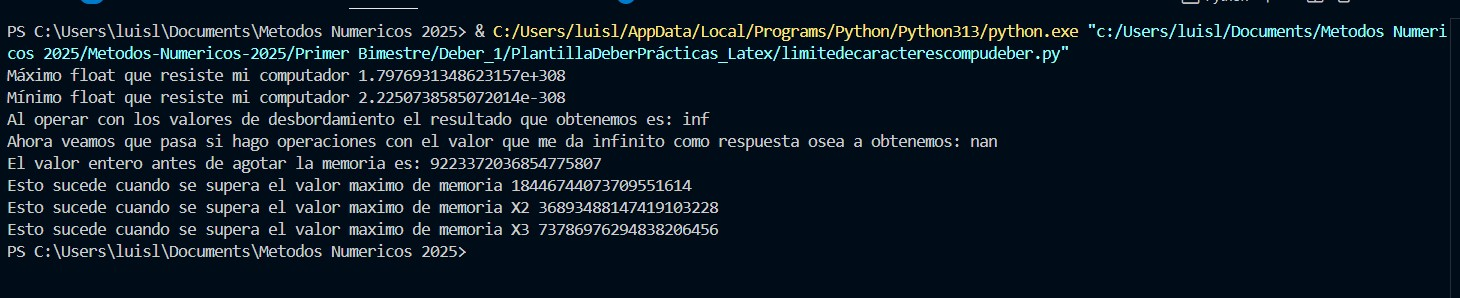
\includegraphics[width=0.95\textwidth]{inFiles/Figures/ej.jpg}
\end{minipage}

\vspace{0.5cm}

\section*{CONCLUSIONES}
\begin{itemize}
    \item { En el ejercicio realizado en python se analizo el error por desbordamiento ya que al obtener el numero máximo y mínimo
    y forzar el desbordamiento se observo como el lenguaje al momento de intentarlo nos de volvió una variable inf que representa un número infinito, al momento de operar con ellos nos dio
    otra variable con nombre nan que tiene como significado (no es un 
    número) y al momento de solicitar el máximo entero antes de llenar la memoria nos da un numero entero arbitrario ya que esto lo comprabamos al operar con el por ello se concluye que el lenguaje de python no permite un error por desbordamiento}
\end{itemize}


\vspace{0.5cm}


\end{document}
